\documentclass[a4paper, 10pt, twoside]{article}
\usepackage[left=2cm, right=2cm, top=2cm, bottom=3cm]{geometry}
\usepackage[super]{natbib}
\usepackage{amsmath}
\usepackage[shortlabels]{enumitem}
\usepackage{bbold}
\usepackage{graphicx}
\usepackage{url}
\usepackage{hyperref}
\hypersetup{
    colorlinks=true,
    linkcolor=blue,
    filecolor=magenta,      
    urlcolor=cyan,
}

\begin{document}

\title{High Performance Computing - Micro Aevol}
\author{T\'eo Bouvard}
\maketitle

\section{Introduction}
\section{Version CPU}
\subsection{Analyse}
Afin de se familiariser avec le code, il est intéressant de profiler son exécution. Cela permet d'identifier la structure globale du programme ainsi que son chemin critique. Dans le cas d'Aevol, on remarque que la fonction \textit{run\_a\_step} est exécutée pour chaque époque, dont le nombre d'itérations est spécifiée par l'argument \textit{n\_steps}.
Dans cette fonction, les différentes étapes du modèle biologique sont exécutées successivement pour chaque organisme. Toutes les étapes de ce modèle sont indépendantes pour chaque organisme sauf l'étape de sélection qui requiert la lecture de l'état des organismes voisins. Une optimisation naturelle est donc de paralléliser le traitement de chaque organisme\label{parallel/orga}.
TODO talk about printf
\subsection{Implémentation}
\hyperref[parallel/orga]{Parallélisation du cycle d'évolution}

\begin{figure}
	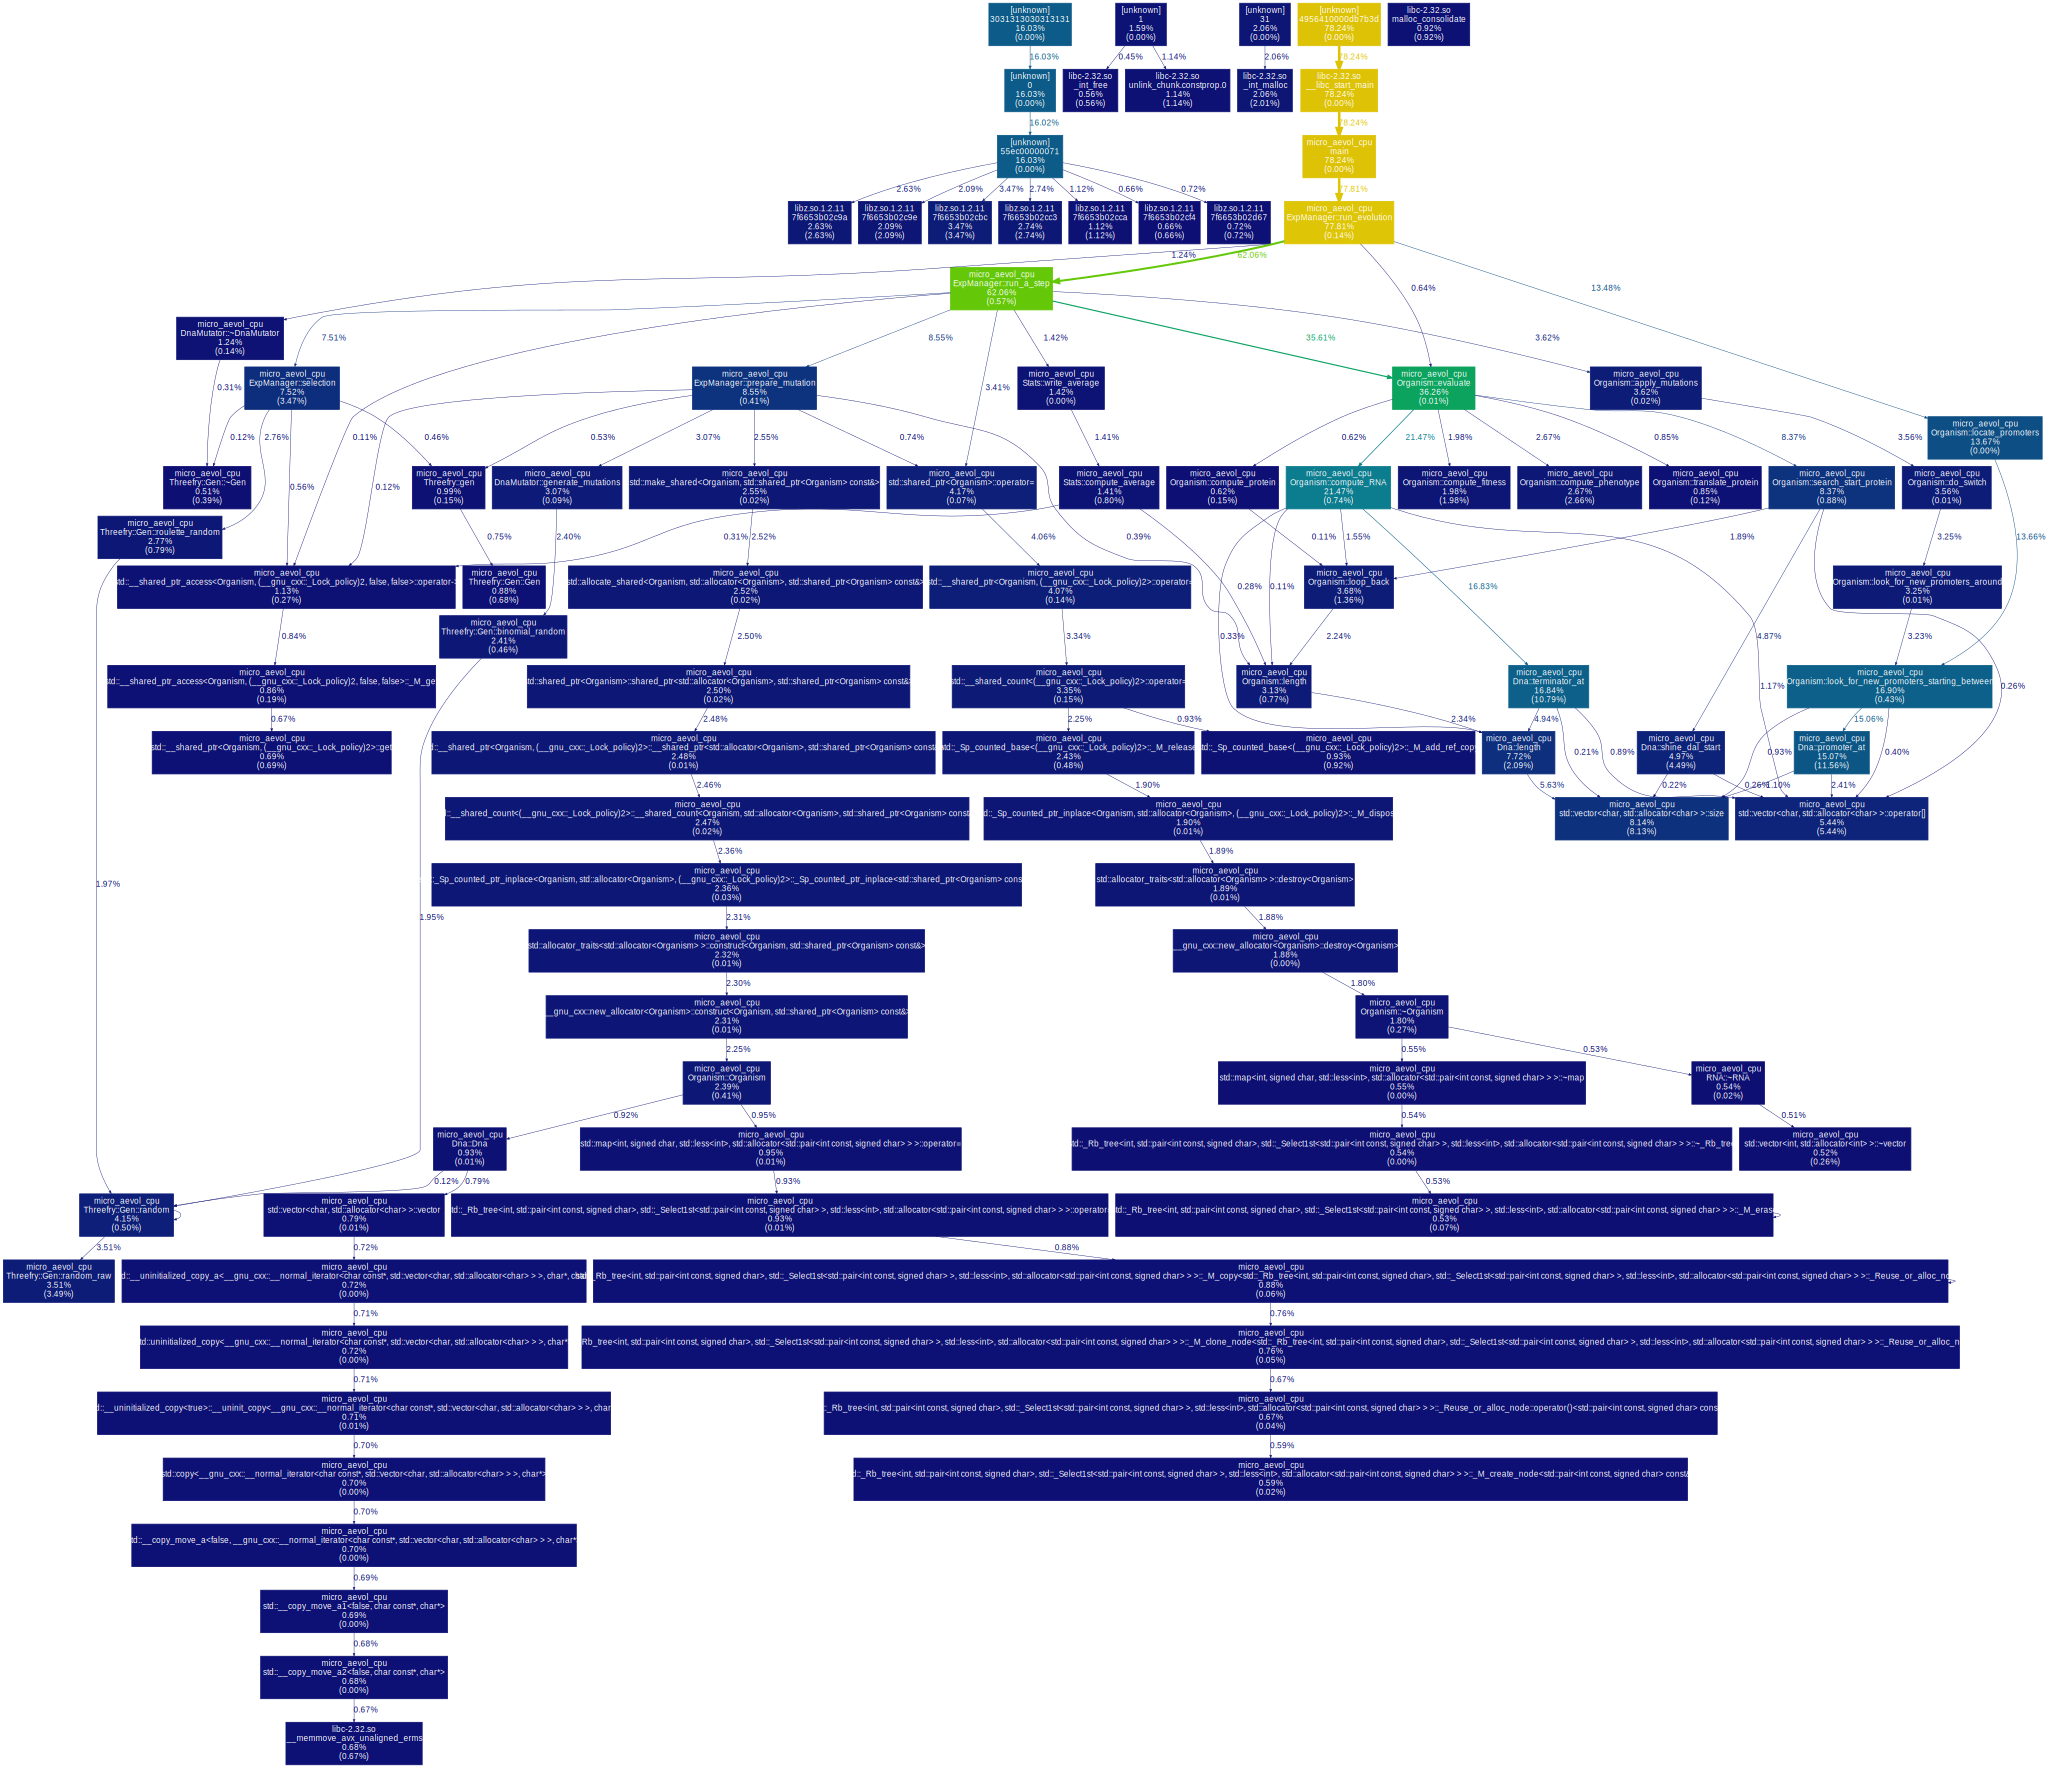
\includegraphics[width=\linewidth]{img/init_profile_debug.png}
\end{figure}
\section{Version GPU}

Divergence \citep{nvidia/branching}



\bibliographystyle{unsrtnat}
\bibliography{report}

\end{document}
